% Created by tikzDevice version 0.10.1 on 2017-11-15 12:08:44
% !TEX encoding = UTF-8 Unicode
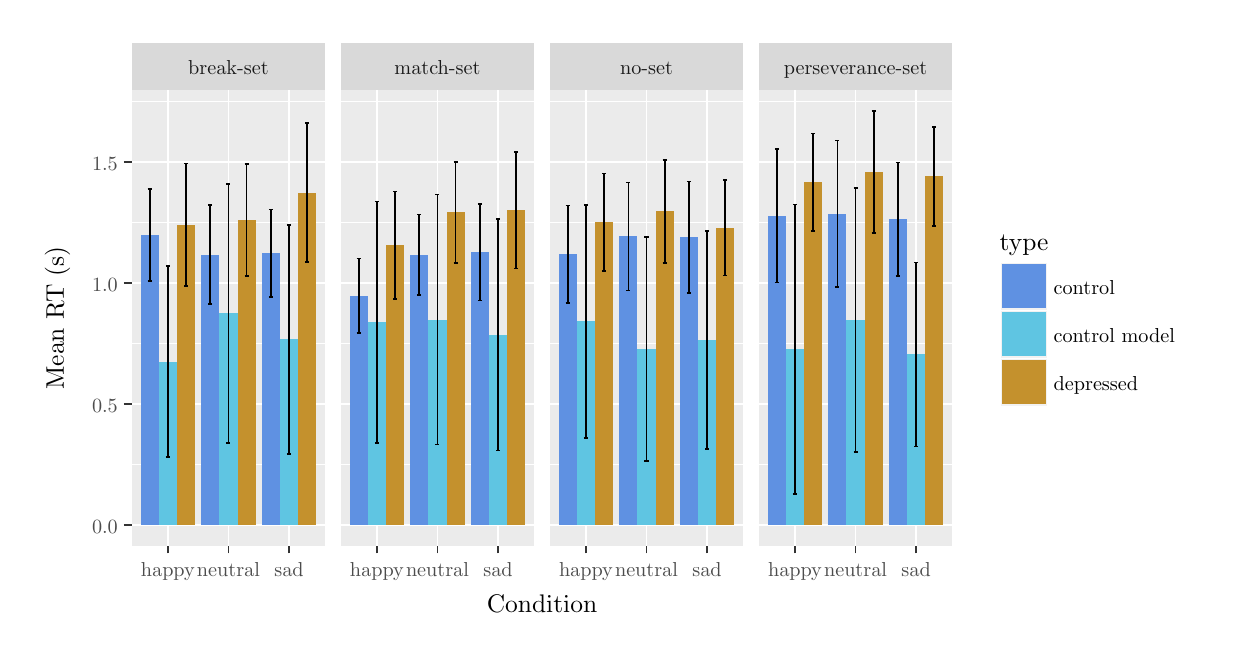
\begin{tikzpicture}[x=1pt,y=1pt]
\definecolor{fillColor}{RGB}{255,255,255}
\path[use as bounding box,fill=fillColor,fill opacity=0.00] (0,0) rectangle (433.62,216.81);
\begin{scope}
\path[clip] (  0.00,  0.00) rectangle (433.62,216.81);
\definecolor{drawColor}{RGB}{255,255,255}
\definecolor{fillColor}{RGB}{255,255,255}

\path[draw=drawColor,line width= 0.6pt,line join=round,line cap=round,fill=fillColor] (  0.00,  0.00) rectangle (433.62,216.81);
\end{scope}
\begin{scope}
\path[clip] ( 37.53, 29.59) rectangle (107.56,194.25);
\definecolor{fillColor}{gray}{0.92}

\path[fill=fillColor] ( 37.53, 29.59) rectangle (107.56,194.25);
\definecolor{drawColor}{RGB}{255,255,255}

\path[draw=drawColor,line width= 0.3pt,line join=round] ( 37.53, 58.93) --
	(107.56, 58.93);

\path[draw=drawColor,line width= 0.3pt,line join=round] ( 37.53,102.65) --
	(107.56,102.65);

\path[draw=drawColor,line width= 0.3pt,line join=round] ( 37.53,146.37) --
	(107.56,146.37);

\path[draw=drawColor,line width= 0.3pt,line join=round] ( 37.53,190.09) --
	(107.56,190.09);

\path[draw=drawColor,line width= 0.6pt,line join=round] ( 37.53, 37.07) --
	(107.56, 37.07);

\path[draw=drawColor,line width= 0.6pt,line join=round] ( 37.53, 80.79) --
	(107.56, 80.79);

\path[draw=drawColor,line width= 0.6pt,line join=round] ( 37.53,124.51) --
	(107.56,124.51);

\path[draw=drawColor,line width= 0.6pt,line join=round] ( 37.53,168.23) --
	(107.56,168.23);

\path[draw=drawColor,line width= 0.6pt,line join=round] ( 50.66, 29.59) --
	( 50.66,194.25);

\path[draw=drawColor,line width= 0.6pt,line join=round] ( 72.55, 29.59) --
	( 72.55,194.25);

\path[draw=drawColor,line width= 0.6pt,line join=round] ( 94.43, 29.59) --
	( 94.43,194.25);
\definecolor{fillColor}{RGB}{196,145,45}

\path[fill=fillColor] ( 53.95, 37.07) rectangle ( 60.51,145.58);
\definecolor{fillColor}{RGB}{95,197,226}

\path[fill=fillColor] ( 47.38, 37.07) rectangle ( 53.95, 96.13);
\definecolor{fillColor}{RGB}{95,145,226}

\path[fill=fillColor] ( 40.82, 37.07) rectangle ( 47.38,141.91);
\definecolor{fillColor}{RGB}{196,145,45}

\path[fill=fillColor] ( 75.83, 37.07) rectangle ( 82.40,147.33);
\definecolor{fillColor}{RGB}{95,197,226}

\path[fill=fillColor] ( 69.27, 37.07) rectangle ( 75.83,113.56);
\definecolor{fillColor}{RGB}{95,145,226}

\path[fill=fillColor] ( 62.70, 37.07) rectangle ( 69.27,134.83);
\definecolor{fillColor}{RGB}{196,145,45}

\path[fill=fillColor] ( 97.72, 37.07) rectangle (104.28,157.21);
\definecolor{fillColor}{RGB}{95,197,226}

\path[fill=fillColor] ( 91.15, 37.07) rectangle ( 97.72,104.19);
\definecolor{fillColor}{RGB}{95,145,226}

\path[fill=fillColor] ( 84.59, 37.07) rectangle ( 91.15,135.26);
\definecolor{drawColor}{RGB}{0,0,0}

\path[draw=drawColor,line width= 0.6pt,line join=round] ( 56.50,167.70) --
	( 57.96,167.70);

\path[draw=drawColor,line width= 0.6pt,line join=round] ( 57.23,167.70) --
	( 57.23,123.46);

\path[draw=drawColor,line width= 0.6pt,line join=round] ( 56.50,123.46) --
	( 57.96,123.46);

\path[draw=drawColor,line width= 0.6pt,line join=round] ( 49.93,130.61) --
	( 51.39,130.61);

\path[draw=drawColor,line width= 0.6pt,line join=round] ( 50.66,130.61) --
	( 50.66, 61.64);

\path[draw=drawColor,line width= 0.6pt,line join=round] ( 49.93, 61.64) --
	( 51.39, 61.64);

\path[draw=drawColor,line width= 0.6pt,line join=round] ( 43.37,158.43) --
	( 44.83,158.43);

\path[draw=drawColor,line width= 0.6pt,line join=round] ( 44.10,158.43) --
	( 44.10,125.38);

\path[draw=drawColor,line width= 0.6pt,line join=round] ( 43.37,125.38) --
	( 44.83,125.38);

\path[draw=drawColor,line width= 0.6pt,line join=round] ( 78.38,167.62) --
	( 79.84,167.62);

\path[draw=drawColor,line width= 0.6pt,line join=round] ( 79.11,167.62) --
	( 79.11,127.04);

\path[draw=drawColor,line width= 0.6pt,line join=round] ( 78.38,127.04) --
	( 79.84,127.04);

\path[draw=drawColor,line width= 0.6pt,line join=round] ( 71.82,160.29) --
	( 73.28,160.29);

\path[draw=drawColor,line width= 0.6pt,line join=round] ( 72.55,160.29) --
	( 72.55, 66.82);

\path[draw=drawColor,line width= 0.6pt,line join=round] ( 71.82, 66.82) --
	( 73.28, 66.82);

\path[draw=drawColor,line width= 0.6pt,line join=round] ( 65.25,152.75) --
	( 66.71,152.75);

\path[draw=drawColor,line width= 0.6pt,line join=round] ( 65.98,152.75) --
	( 65.98,116.90);

\path[draw=drawColor,line width= 0.6pt,line join=round] ( 65.25,116.90) --
	( 66.71,116.90);

\path[draw=drawColor,line width= 0.6pt,line join=round] (100.27,182.39) --
	(101.73,182.39);

\path[draw=drawColor,line width= 0.6pt,line join=round] (101.00,182.39) --
	(101.00,132.03);

\path[draw=drawColor,line width= 0.6pt,line join=round] (100.27,132.03) --
	(101.73,132.03);

\path[draw=drawColor,line width= 0.6pt,line join=round] ( 93.70,145.61) --
	( 95.16,145.61);

\path[draw=drawColor,line width= 0.6pt,line join=round] ( 94.43,145.61) --
	( 94.43, 62.77);

\path[draw=drawColor,line width= 0.6pt,line join=round] ( 93.70, 62.77) --
	( 95.16, 62.77);

\path[draw=drawColor,line width= 0.6pt,line join=round] ( 87.14,151.09) --
	( 88.60,151.09);

\path[draw=drawColor,line width= 0.6pt,line join=round] ( 87.87,151.09) --
	( 87.87,119.44);

\path[draw=drawColor,line width= 0.6pt,line join=round] ( 87.14,119.44) --
	( 88.60,119.44);
\end{scope}
\begin{scope}
\path[clip] (113.06, 29.59) rectangle (183.10,194.25);
\definecolor{fillColor}{gray}{0.92}

\path[fill=fillColor] (113.06, 29.59) rectangle (183.10,194.25);
\definecolor{drawColor}{RGB}{255,255,255}

\path[draw=drawColor,line width= 0.3pt,line join=round] (113.06, 58.93) --
	(183.10, 58.93);

\path[draw=drawColor,line width= 0.3pt,line join=round] (113.06,102.65) --
	(183.10,102.65);

\path[draw=drawColor,line width= 0.3pt,line join=round] (113.06,146.37) --
	(183.10,146.37);

\path[draw=drawColor,line width= 0.3pt,line join=round] (113.06,190.09) --
	(183.10,190.09);

\path[draw=drawColor,line width= 0.6pt,line join=round] (113.06, 37.07) --
	(183.10, 37.07);

\path[draw=drawColor,line width= 0.6pt,line join=round] (113.06, 80.79) --
	(183.10, 80.79);

\path[draw=drawColor,line width= 0.6pt,line join=round] (113.06,124.51) --
	(183.10,124.51);

\path[draw=drawColor,line width= 0.6pt,line join=round] (113.06,168.23) --
	(183.10,168.23);

\path[draw=drawColor,line width= 0.6pt,line join=round] (126.20, 29.59) --
	(126.20,194.25);

\path[draw=drawColor,line width= 0.6pt,line join=round] (148.08, 29.59) --
	(148.08,194.25);

\path[draw=drawColor,line width= 0.6pt,line join=round] (169.97, 29.59) --
	(169.97,194.25);
\definecolor{fillColor}{RGB}{196,145,45}

\path[fill=fillColor] (129.48, 37.07) rectangle (136.04,138.15);
\definecolor{fillColor}{RGB}{95,197,226}

\path[fill=fillColor] (122.91, 37.07) rectangle (129.48,110.32);
\definecolor{fillColor}{RGB}{95,145,226}

\path[fill=fillColor] (116.35, 37.07) rectangle (122.91,119.96);
\definecolor{fillColor}{RGB}{196,145,45}

\path[fill=fillColor] (151.36, 37.07) rectangle (157.93,150.04);
\definecolor{fillColor}{RGB}{95,197,226}

\path[fill=fillColor] (144.80, 37.07) rectangle (151.36,111.31);
\definecolor{fillColor}{RGB}{95,145,226}

\path[fill=fillColor] (138.23, 37.07) rectangle (144.80,134.74);
\definecolor{fillColor}{RGB}{196,145,45}

\path[fill=fillColor] (173.25, 37.07) rectangle (179.81,150.92);
\definecolor{fillColor}{RGB}{95,197,226}

\path[fill=fillColor] (166.68, 37.07) rectangle (173.25,105.83);
\definecolor{fillColor}{RGB}{95,145,226}

\path[fill=fillColor] (160.12, 37.07) rectangle (166.68,135.61);
\definecolor{drawColor}{RGB}{0,0,0}

\path[draw=drawColor,line width= 0.6pt,line join=round] (132.03,157.56) --
	(133.49,157.56);

\path[draw=drawColor,line width= 0.6pt,line join=round] (132.76,157.56) --
	(132.76,118.74);

\path[draw=drawColor,line width= 0.6pt,line join=round] (132.03,118.74) --
	(133.49,118.74);

\path[draw=drawColor,line width= 0.6pt,line join=round] (125.47,153.95) --
	(126.92,153.95);

\path[draw=drawColor,line width= 0.6pt,line join=round] (126.20,153.95) --
	(126.20, 66.69);

\path[draw=drawColor,line width= 0.6pt,line join=round] (125.47, 66.69) --
	(126.92, 66.69);

\path[draw=drawColor,line width= 0.6pt,line join=round] (118.90,133.43) --
	(120.36,133.43);

\path[draw=drawColor,line width= 0.6pt,line join=round] (119.63,133.43) --
	(119.63,106.50);

\path[draw=drawColor,line width= 0.6pt,line join=round] (118.90,106.50) --
	(120.36,106.50);

\path[draw=drawColor,line width= 0.6pt,line join=round] (153.92,168.32) --
	(155.38,168.32);

\path[draw=drawColor,line width= 0.6pt,line join=round] (154.65,168.32) --
	(154.65,131.77);

\path[draw=drawColor,line width= 0.6pt,line join=round] (153.92,131.77) --
	(155.38,131.77);

\path[draw=drawColor,line width= 0.6pt,line join=round] (147.35,156.48) --
	(148.81,156.48);

\path[draw=drawColor,line width= 0.6pt,line join=round] (148.08,156.48) --
	(148.08, 66.13);

\path[draw=drawColor,line width= 0.6pt,line join=round] (147.35, 66.13) --
	(148.81, 66.13);

\path[draw=drawColor,line width= 0.6pt,line join=round] (140.79,149.34) --
	(142.24,149.34);

\path[draw=drawColor,line width= 0.6pt,line join=round] (141.51,149.34) --
	(141.51,120.14);

\path[draw=drawColor,line width= 0.6pt,line join=round] (140.79,120.14) --
	(142.24,120.14);

\path[draw=drawColor,line width= 0.6pt,line join=round] (175.80,171.99) --
	(177.26,171.99);

\path[draw=drawColor,line width= 0.6pt,line join=round] (176.53,171.99) --
	(176.53,129.84);

\path[draw=drawColor,line width= 0.6pt,line join=round] (175.80,129.84) --
	(177.26,129.84);

\path[draw=drawColor,line width= 0.6pt,line join=round] (169.24,147.69) --
	(170.69,147.69);

\path[draw=drawColor,line width= 0.6pt,line join=round] (169.97,147.69) --
	(169.97, 63.97);

\path[draw=drawColor,line width= 0.6pt,line join=round] (169.24, 63.97) --
	(170.69, 63.97);

\path[draw=drawColor,line width= 0.6pt,line join=round] (162.67,153.01) --
	(164.13,153.01);

\path[draw=drawColor,line width= 0.6pt,line join=round] (163.40,153.01) --
	(163.40,118.21);

\path[draw=drawColor,line width= 0.6pt,line join=round] (162.67,118.21) --
	(164.13,118.21);
\end{scope}
\begin{scope}
\path[clip] (188.60, 29.59) rectangle (258.63,194.25);
\definecolor{fillColor}{gray}{0.92}

\path[fill=fillColor] (188.60, 29.59) rectangle (258.63,194.25);
\definecolor{drawColor}{RGB}{255,255,255}

\path[draw=drawColor,line width= 0.3pt,line join=round] (188.60, 58.93) --
	(258.63, 58.93);

\path[draw=drawColor,line width= 0.3pt,line join=round] (188.60,102.65) --
	(258.63,102.65);

\path[draw=drawColor,line width= 0.3pt,line join=round] (188.60,146.37) --
	(258.63,146.37);

\path[draw=drawColor,line width= 0.3pt,line join=round] (188.60,190.09) --
	(258.63,190.09);

\path[draw=drawColor,line width= 0.6pt,line join=round] (188.60, 37.07) --
	(258.63, 37.07);

\path[draw=drawColor,line width= 0.6pt,line join=round] (188.60, 80.79) --
	(258.63, 80.79);

\path[draw=drawColor,line width= 0.6pt,line join=round] (188.60,124.51) --
	(258.63,124.51);

\path[draw=drawColor,line width= 0.6pt,line join=round] (188.60,168.23) --
	(258.63,168.23);

\path[draw=drawColor,line width= 0.6pt,line join=round] (201.73, 29.59) --
	(201.73,194.25);

\path[draw=drawColor,line width= 0.6pt,line join=round] (223.61, 29.59) --
	(223.61,194.25);

\path[draw=drawColor,line width= 0.6pt,line join=round] (245.50, 29.59) --
	(245.50,194.25);
\definecolor{fillColor}{RGB}{196,145,45}

\path[fill=fillColor] (205.01, 37.07) rectangle (211.58,146.46);
\definecolor{fillColor}{RGB}{95,197,226}

\path[fill=fillColor] (198.44, 37.07) rectangle (205.01,110.66);
\definecolor{fillColor}{RGB}{95,145,226}

\path[fill=fillColor] (191.88, 37.07) rectangle (198.44,134.91);
\definecolor{fillColor}{RGB}{196,145,45}

\path[fill=fillColor] (226.89, 37.07) rectangle (233.46,150.39);
\definecolor{fillColor}{RGB}{95,197,226}

\path[fill=fillColor] (220.33, 37.07) rectangle (226.89,100.74);
\definecolor{fillColor}{RGB}{95,145,226}

\path[fill=fillColor] (213.76, 37.07) rectangle (220.33,141.38);
\definecolor{fillColor}{RGB}{196,145,45}

\path[fill=fillColor] (248.78, 37.07) rectangle (255.34,144.44);
\definecolor{fillColor}{RGB}{95,197,226}

\path[fill=fillColor] (242.21, 37.07) rectangle (248.78,103.92);
\definecolor{fillColor}{RGB}{95,145,226}

\path[fill=fillColor] (235.65, 37.07) rectangle (242.21,141.12);
\definecolor{drawColor}{RGB}{0,0,0}

\path[draw=drawColor,line width= 0.6pt,line join=round] (207.56,164.12) --
	(209.02,164.12);

\path[draw=drawColor,line width= 0.6pt,line join=round] (208.29,164.12) --
	(208.29,128.79);

\path[draw=drawColor,line width= 0.6pt,line join=round] (207.56,128.79) --
	(209.02,128.79);

\path[draw=drawColor,line width= 0.6pt,line join=round] (201.00,152.79) --
	(202.46,152.79);

\path[draw=drawColor,line width= 0.6pt,line join=round] (201.73,152.79) --
	(201.73, 68.53);

\path[draw=drawColor,line width= 0.6pt,line join=round] (201.00, 68.53) --
	(202.46, 68.53);

\path[draw=drawColor,line width= 0.6pt,line join=round] (194.43,152.49) --
	(195.89,152.49);

\path[draw=drawColor,line width= 0.6pt,line join=round] (195.16,152.49) --
	(195.16,117.34);

\path[draw=drawColor,line width= 0.6pt,line join=round] (194.43,117.34) --
	(195.89,117.34);

\path[draw=drawColor,line width= 0.6pt,line join=round] (229.45,168.93) --
	(230.91,168.93);

\path[draw=drawColor,line width= 0.6pt,line join=round] (230.18,168.93) --
	(230.18,131.85);

\path[draw=drawColor,line width= 0.6pt,line join=round] (229.45,131.85) --
	(230.91,131.85);

\path[draw=drawColor,line width= 0.6pt,line join=round] (222.88,141.14) --
	(224.34,141.14);

\path[draw=drawColor,line width= 0.6pt,line join=round] (223.61,141.14) --
	(223.61, 60.34);

\path[draw=drawColor,line width= 0.6pt,line join=round] (222.88, 60.34) --
	(224.34, 60.34);

\path[draw=drawColor,line width= 0.6pt,line join=round] (216.32,160.88) --
	(217.78,160.88);

\path[draw=drawColor,line width= 0.6pt,line join=round] (217.05,160.88) --
	(217.05,121.89);

\path[draw=drawColor,line width= 0.6pt,line join=round] (216.32,121.89) --
	(217.78,121.89);

\path[draw=drawColor,line width= 0.6pt,line join=round] (251.33,161.67) --
	(252.79,161.67);

\path[draw=drawColor,line width= 0.6pt,line join=round] (252.06,161.67) --
	(252.06,127.22);

\path[draw=drawColor,line width= 0.6pt,line join=round] (251.33,127.22) --
	(252.79,127.22);

\path[draw=drawColor,line width= 0.6pt,line join=round] (244.77,143.24) --
	(246.23,143.24);

\path[draw=drawColor,line width= 0.6pt,line join=round] (245.50,143.24) --
	(245.50, 64.59);

\path[draw=drawColor,line width= 0.6pt,line join=round] (244.77, 64.59) --
	(246.23, 64.59);

\path[draw=drawColor,line width= 0.6pt,line join=round] (238.20,161.23) --
	(239.66,161.23);

\path[draw=drawColor,line width= 0.6pt,line join=round] (238.93,161.23) --
	(238.93,121.01);

\path[draw=drawColor,line width= 0.6pt,line join=round] (238.20,121.01) --
	(239.66,121.01);
\end{scope}
\begin{scope}
\path[clip] (264.13, 29.59) rectangle (334.16,194.25);
\definecolor{fillColor}{gray}{0.92}

\path[fill=fillColor] (264.13, 29.59) rectangle (334.16,194.25);
\definecolor{drawColor}{RGB}{255,255,255}

\path[draw=drawColor,line width= 0.3pt,line join=round] (264.13, 58.93) --
	(334.16, 58.93);

\path[draw=drawColor,line width= 0.3pt,line join=round] (264.13,102.65) --
	(334.16,102.65);

\path[draw=drawColor,line width= 0.3pt,line join=round] (264.13,146.37) --
	(334.16,146.37);

\path[draw=drawColor,line width= 0.3pt,line join=round] (264.13,190.09) --
	(334.16,190.09);

\path[draw=drawColor,line width= 0.6pt,line join=round] (264.13, 37.07) --
	(334.16, 37.07);

\path[draw=drawColor,line width= 0.6pt,line join=round] (264.13, 80.79) --
	(334.16, 80.79);

\path[draw=drawColor,line width= 0.6pt,line join=round] (264.13,124.51) --
	(334.16,124.51);

\path[draw=drawColor,line width= 0.6pt,line join=round] (264.13,168.23) --
	(334.16,168.23);

\path[draw=drawColor,line width= 0.6pt,line join=round] (277.26, 29.59) --
	(277.26,194.25);

\path[draw=drawColor,line width= 0.6pt,line join=round] (299.14, 29.59) --
	(299.14,194.25);

\path[draw=drawColor,line width= 0.6pt,line join=round] (321.03, 29.59) --
	(321.03,194.25);
\definecolor{fillColor}{RGB}{196,145,45}

\path[fill=fillColor] (280.54, 37.07) rectangle (287.11,160.97);
\definecolor{fillColor}{RGB}{95,197,226}

\path[fill=fillColor] (273.98, 37.07) rectangle (280.54,100.63);
\definecolor{fillColor}{RGB}{95,145,226}

\path[fill=fillColor] (267.41, 37.07) rectangle (273.98,148.82);
\definecolor{fillColor}{RGB}{196,145,45}

\path[fill=fillColor] (302.43, 37.07) rectangle (308.99,164.73);
\definecolor{fillColor}{RGB}{95,197,226}

\path[fill=fillColor] (295.86, 37.07) rectangle (302.43,111.21);
\definecolor{fillColor}{RGB}{95,145,226}

\path[fill=fillColor] (289.30, 37.07) rectangle (295.86,149.52);
\definecolor{fillColor}{RGB}{196,145,45}

\path[fill=fillColor] (324.31, 37.07) rectangle (330.88,163.07);
\definecolor{fillColor}{RGB}{95,197,226}

\path[fill=fillColor] (317.75, 37.07) rectangle (324.31, 98.71);
\definecolor{fillColor}{RGB}{95,145,226}

\path[fill=fillColor] (311.18, 37.07) rectangle (317.75,147.51);
\definecolor{drawColor}{RGB}{0,0,0}

\path[draw=drawColor,line width= 0.6pt,line join=round] (283.09,178.55) --
	(284.55,178.55);

\path[draw=drawColor,line width= 0.6pt,line join=round] (283.82,178.55) --
	(283.82,143.40);

\path[draw=drawColor,line width= 0.6pt,line join=round] (283.09,143.40) --
	(284.55,143.40);

\path[draw=drawColor,line width= 0.6pt,line join=round] (276.53,152.85) --
	(277.99,152.85);

\path[draw=drawColor,line width= 0.6pt,line join=round] (277.26,152.85) --
	(277.26, 48.40);

\path[draw=drawColor,line width= 0.6pt,line join=round] (276.53, 48.40) --
	(277.99, 48.40);

\path[draw=drawColor,line width= 0.6pt,line join=round] (269.96,172.95) --
	(271.42,172.95);

\path[draw=drawColor,line width= 0.6pt,line join=round] (270.69,172.95) --
	(270.69,124.68);

\path[draw=drawColor,line width= 0.6pt,line join=round] (269.96,124.68) --
	(271.42,124.68);

\path[draw=drawColor,line width= 0.6pt,line join=round] (304.98,186.76) --
	(306.44,186.76);

\path[draw=drawColor,line width= 0.6pt,line join=round] (305.71,186.76) --
	(305.71,142.70);

\path[draw=drawColor,line width= 0.6pt,line join=round] (304.98,142.70) --
	(306.44,142.70);

\path[draw=drawColor,line width= 0.6pt,line join=round] (298.41,158.85) --
	(299.87,158.85);

\path[draw=drawColor,line width= 0.6pt,line join=round] (299.14,158.85) --
	(299.14, 63.57);

\path[draw=drawColor,line width= 0.6pt,line join=round] (298.41, 63.57) --
	(299.87, 63.57);

\path[draw=drawColor,line width= 0.6pt,line join=round] (291.85,176.01) --
	(293.31,176.01);

\path[draw=drawColor,line width= 0.6pt,line join=round] (292.58,176.01) --
	(292.58,123.02);

\path[draw=drawColor,line width= 0.6pt,line join=round] (291.85,123.02) --
	(293.31,123.02);

\path[draw=drawColor,line width= 0.6pt,line join=round] (326.86,180.99) --
	(328.32,180.99);

\path[draw=drawColor,line width= 0.6pt,line join=round] (327.59,180.99) --
	(327.59,145.14);

\path[draw=drawColor,line width= 0.6pt,line join=round] (326.86,145.14) --
	(328.32,145.14);

\path[draw=drawColor,line width= 0.6pt,line join=round] (320.30,132.00) --
	(321.76,132.00);

\path[draw=drawColor,line width= 0.6pt,line join=round] (321.03,132.00) --
	(321.03, 65.42);

\path[draw=drawColor,line width= 0.6pt,line join=round] (320.30, 65.42) --
	(321.76, 65.42);

\path[draw=drawColor,line width= 0.6pt,line join=round] (313.73,168.05) --
	(315.19,168.05);

\path[draw=drawColor,line width= 0.6pt,line join=round] (314.46,168.05) --
	(314.46,126.96);

\path[draw=drawColor,line width= 0.6pt,line join=round] (313.73,126.96) --
	(315.19,126.96);
\end{scope}
\begin{scope}
\path[clip] ( 37.53,194.25) rectangle (107.56,211.31);
\definecolor{fillColor}{gray}{0.85}

\path[fill=fillColor] ( 37.53,194.25) rectangle (107.56,211.31);
\definecolor{drawColor}{gray}{0.10}

\node[text=drawColor,anchor=base,inner sep=0pt, outer sep=0pt, scale=  0.73] at ( 72.55,199.75) {break-set};
\end{scope}
\begin{scope}
\path[clip] (113.06,194.25) rectangle (183.10,211.31);
\definecolor{fillColor}{gray}{0.85}

\path[fill=fillColor] (113.06,194.25) rectangle (183.10,211.31);
\definecolor{drawColor}{gray}{0.10}

\node[text=drawColor,anchor=base,inner sep=0pt, outer sep=0pt, scale=  0.73] at (148.08,199.75) {match-set};
\end{scope}
\begin{scope}
\path[clip] (188.60,194.25) rectangle (258.63,211.31);
\definecolor{fillColor}{gray}{0.85}

\path[fill=fillColor] (188.60,194.25) rectangle (258.63,211.31);
\definecolor{drawColor}{gray}{0.10}

\node[text=drawColor,anchor=base,inner sep=0pt, outer sep=0pt, scale=  0.73] at (223.61,199.75) {no-set};
\end{scope}
\begin{scope}
\path[clip] (264.13,194.25) rectangle (334.16,211.31);
\definecolor{fillColor}{gray}{0.85}

\path[fill=fillColor] (264.13,194.25) rectangle (334.16,211.31);
\definecolor{drawColor}{gray}{0.10}

\node[text=drawColor,anchor=base,inner sep=0pt, outer sep=0pt, scale=  0.73] at (299.14,199.75) {perseverance-set};
\end{scope}
\begin{scope}
\path[clip] (  0.00,  0.00) rectangle (433.62,216.81);
\definecolor{drawColor}{gray}{0.20}

\path[draw=drawColor,line width= 0.6pt,line join=round] ( 50.66, 26.84) --
	( 50.66, 29.59);

\path[draw=drawColor,line width= 0.6pt,line join=round] ( 72.55, 26.84) --
	( 72.55, 29.59);

\path[draw=drawColor,line width= 0.6pt,line join=round] ( 94.43, 26.84) --
	( 94.43, 29.59);
\end{scope}
\begin{scope}
\path[clip] (  0.00,  0.00) rectangle (433.62,216.81);
\definecolor{drawColor}{gray}{0.30}

\node[text=drawColor,anchor=base,inner sep=0pt, outer sep=0pt, scale=  0.73] at ( 50.66, 18.58) {happy};

\node[text=drawColor,anchor=base,inner sep=0pt, outer sep=0pt, scale=  0.73] at ( 72.55, 18.58) {neutral};

\node[text=drawColor,anchor=base,inner sep=0pt, outer sep=0pt, scale=  0.73] at ( 94.43, 18.58) {sad};
\end{scope}
\begin{scope}
\path[clip] (  0.00,  0.00) rectangle (433.62,216.81);
\definecolor{drawColor}{gray}{0.20}

\path[draw=drawColor,line width= 0.6pt,line join=round] (126.20, 26.84) --
	(126.20, 29.59);

\path[draw=drawColor,line width= 0.6pt,line join=round] (148.08, 26.84) --
	(148.08, 29.59);

\path[draw=drawColor,line width= 0.6pt,line join=round] (169.97, 26.84) --
	(169.97, 29.59);
\end{scope}
\begin{scope}
\path[clip] (  0.00,  0.00) rectangle (433.62,216.81);
\definecolor{drawColor}{gray}{0.30}

\node[text=drawColor,anchor=base,inner sep=0pt, outer sep=0pt, scale=  0.73] at (126.20, 18.58) {happy};

\node[text=drawColor,anchor=base,inner sep=0pt, outer sep=0pt, scale=  0.73] at (148.08, 18.58) {neutral};

\node[text=drawColor,anchor=base,inner sep=0pt, outer sep=0pt, scale=  0.73] at (169.97, 18.58) {sad};
\end{scope}
\begin{scope}
\path[clip] (  0.00,  0.00) rectangle (433.62,216.81);
\definecolor{drawColor}{gray}{0.20}

\path[draw=drawColor,line width= 0.6pt,line join=round] (201.73, 26.84) --
	(201.73, 29.59);

\path[draw=drawColor,line width= 0.6pt,line join=round] (223.61, 26.84) --
	(223.61, 29.59);

\path[draw=drawColor,line width= 0.6pt,line join=round] (245.50, 26.84) --
	(245.50, 29.59);
\end{scope}
\begin{scope}
\path[clip] (  0.00,  0.00) rectangle (433.62,216.81);
\definecolor{drawColor}{gray}{0.30}

\node[text=drawColor,anchor=base,inner sep=0pt, outer sep=0pt, scale=  0.73] at (201.73, 18.58) {happy};

\node[text=drawColor,anchor=base,inner sep=0pt, outer sep=0pt, scale=  0.73] at (223.61, 18.58) {neutral};

\node[text=drawColor,anchor=base,inner sep=0pt, outer sep=0pt, scale=  0.73] at (245.50, 18.58) {sad};
\end{scope}
\begin{scope}
\path[clip] (  0.00,  0.00) rectangle (433.62,216.81);
\definecolor{drawColor}{gray}{0.20}

\path[draw=drawColor,line width= 0.6pt,line join=round] (277.26, 26.84) --
	(277.26, 29.59);

\path[draw=drawColor,line width= 0.6pt,line join=round] (299.14, 26.84) --
	(299.14, 29.59);

\path[draw=drawColor,line width= 0.6pt,line join=round] (321.03, 26.84) --
	(321.03, 29.59);
\end{scope}
\begin{scope}
\path[clip] (  0.00,  0.00) rectangle (433.62,216.81);
\definecolor{drawColor}{gray}{0.30}

\node[text=drawColor,anchor=base,inner sep=0pt, outer sep=0pt, scale=  0.73] at (277.26, 18.58) {happy};

\node[text=drawColor,anchor=base,inner sep=0pt, outer sep=0pt, scale=  0.73] at (299.14, 18.58) {neutral};

\node[text=drawColor,anchor=base,inner sep=0pt, outer sep=0pt, scale=  0.73] at (321.03, 18.58) {sad};
\end{scope}
\begin{scope}
\path[clip] (  0.00,  0.00) rectangle (433.62,216.81);
\definecolor{drawColor}{gray}{0.30}

\node[text=drawColor,anchor=base east,inner sep=0pt, outer sep=0pt, scale=  0.73] at ( 32.58, 34.04) {0.0};

\node[text=drawColor,anchor=base east,inner sep=0pt, outer sep=0pt, scale=  0.73] at ( 32.58, 77.76) {0.5};

\node[text=drawColor,anchor=base east,inner sep=0pt, outer sep=0pt, scale=  0.73] at ( 32.58,121.48) {1.0};

\node[text=drawColor,anchor=base east,inner sep=0pt, outer sep=0pt, scale=  0.73] at ( 32.58,165.20) {1.5};
\end{scope}
\begin{scope}
\path[clip] (  0.00,  0.00) rectangle (433.62,216.81);
\definecolor{drawColor}{gray}{0.20}

\path[draw=drawColor,line width= 0.6pt,line join=round] ( 34.78, 37.07) --
	( 37.53, 37.07);

\path[draw=drawColor,line width= 0.6pt,line join=round] ( 34.78, 80.79) --
	( 37.53, 80.79);

\path[draw=drawColor,line width= 0.6pt,line join=round] ( 34.78,124.51) --
	( 37.53,124.51);

\path[draw=drawColor,line width= 0.6pt,line join=round] ( 34.78,168.23) --
	( 37.53,168.23);
\end{scope}
\begin{scope}
\path[clip] (  0.00,  0.00) rectangle (433.62,216.81);
\definecolor{drawColor}{RGB}{0,0,0}

\node[text=drawColor,anchor=base,inner sep=0pt, outer sep=0pt, scale=  0.92] at (185.85,  5.50) {Condition};
\end{scope}
\begin{scope}
\path[clip] (  0.00,  0.00) rectangle (433.62,216.81);
\definecolor{drawColor}{RGB}{0,0,0}

\node[text=drawColor,rotate= 90.00,anchor=base,inner sep=0pt, outer sep=0pt, scale=  0.92] at ( 13.08,111.92) {Mean RT (s)};
\end{scope}
\begin{scope}
\path[clip] (  0.00,  0.00) rectangle (433.62,216.81);
\definecolor{fillColor}{RGB}{255,255,255}

\path[fill=fillColor] (345.54, 74.25) rectangle (428.12,149.58);
\end{scope}
\begin{scope}
\path[clip] (  0.00,  0.00) rectangle (433.62,216.81);
\definecolor{drawColor}{RGB}{0,0,0}

\node[text=drawColor,anchor=base west,inner sep=0pt, outer sep=0pt, scale=  0.92] at (351.23,136.32) {type};
\end{scope}
\begin{scope}
\path[clip] (  0.00,  0.00) rectangle (433.62,216.81);
\definecolor{drawColor}{RGB}{255,255,255}
\definecolor{fillColor}{gray}{0.95}

\path[draw=drawColor,line width= 0.6pt,line join=round,line cap=round,fill=fillColor] (351.23,114.63) rectangle (368.58,131.98);
\end{scope}
\begin{scope}
\path[clip] (  0.00,  0.00) rectangle (433.62,216.81);
\definecolor{fillColor}{RGB}{95,145,226}

\path[fill=fillColor] (351.94,115.35) rectangle (367.86,131.27);
\end{scope}
\begin{scope}
\path[clip] (  0.00,  0.00) rectangle (433.62,216.81);
\definecolor{drawColor}{RGB}{255,255,255}
\definecolor{fillColor}{gray}{0.95}

\path[draw=drawColor,line width= 0.6pt,line join=round,line cap=round,fill=fillColor] (351.23, 97.29) rectangle (368.58,114.63);
\end{scope}
\begin{scope}
\path[clip] (  0.00,  0.00) rectangle (433.62,216.81);
\definecolor{fillColor}{RGB}{95,197,226}

\path[fill=fillColor] (351.94, 98.00) rectangle (367.86,113.92);
\end{scope}
\begin{scope}
\path[clip] (  0.00,  0.00) rectangle (433.62,216.81);
\definecolor{drawColor}{RGB}{255,255,255}
\definecolor{fillColor}{gray}{0.95}

\path[draw=drawColor,line width= 0.6pt,line join=round,line cap=round,fill=fillColor] (351.23, 79.94) rectangle (368.58, 97.29);
\end{scope}
\begin{scope}
\path[clip] (  0.00,  0.00) rectangle (433.62,216.81);
\definecolor{fillColor}{RGB}{196,145,45}

\path[fill=fillColor] (351.94, 80.66) rectangle (367.86, 96.58);
\end{scope}
\begin{scope}
\path[clip] (  0.00,  0.00) rectangle (433.62,216.81);
\definecolor{drawColor}{RGB}{0,0,0}

\node[text=drawColor,anchor=base west,inner sep=0pt, outer sep=0pt, scale=  0.73] at (370.74,120.28) {control};
\end{scope}
\begin{scope}
\path[clip] (  0.00,  0.00) rectangle (433.62,216.81);
\definecolor{drawColor}{RGB}{0,0,0}

\node[text=drawColor,anchor=base west,inner sep=0pt, outer sep=0pt, scale=  0.73] at (370.74,102.93) {control model};
\end{scope}
\begin{scope}
\path[clip] (  0.00,  0.00) rectangle (433.62,216.81);
\definecolor{drawColor}{RGB}{0,0,0}

\node[text=drawColor,anchor=base west,inner sep=0pt, outer sep=0pt, scale=  0.73] at (370.74, 85.59) {depressed};
\end{scope}
\end{tikzpicture}
